\documentclass{article}

\usepackage[T1]{fontenc}
\usepackage[utf8]{inputenc}
\usepackage{graphicx}
\usepackage[font=small,labelfont=bf]{caption}
\usepackage{booktabs, siunitx}
\usepackage{tikz}
\usepackage{tikz-qtree}
\usepackage{pifont}
\usepackage[margin=0.90in]{geometry}
\usepackage{etoolbox,titling}
\usepackage{enumitem}
\usepackage{fancyhdr}
\usepackage{soulutf8}

\pagestyle{fancy}
\fancyhf{}
\rhead{Chiara Solito}
\lhead{Dispense di Laboratorio di Bioinformatica}
\rfoot{Pagina \thepage}
\lfoot{Bioinformatica - A.A. 2021/22}
\usetikzlibrary{trees}
\tikzstyle{every node}=[draw=black,thick,anchor=west]


\begin{document}
\newcommand\tab[1][0.3cm]{\hspace*{#1}}


\begin{titlepage}
    \begin{center}
        \vspace*{1cm}
            
        \Huge
        \textbf{Laboratorio di Bioinformatica}
            
        \vspace{0.5cm}
        \LARGE
        Dispense del corso
            
        \vspace{1.5cm}
            
        \textbf{Chiara Solito}

        \vspace{0.8cm}

            
        \Large
        Corso di Laurea in Bioinformatica\\
        Università degli studi di Verona\\
        A.A. 2021/22
            
    \end{center}
\end{titlepage}
La presente è una dispensa riguardante il corso di \textbf{Laboratorio di Bioinformatica} del CdS in Bioinformatica (Università degli Studi di Verona). Per la stesura di questa dispensa si è fatta fede al materiale didattico fornito direttamente dal professore nell'Anno Accademico 2021/2022. Eventuali variazioni al programma successive al suddetto anno non saranno quindi incluse.\\
Insieme a questo documento in formato PDF viene fornito anche il codice \LaTeX  con cui è stato generato.
\tableofcontents
\thispagestyle{empty}
\newpage
\thispagestyle{empty}
\section{Il corso}
Il corso si propone di presentare allo studente le basi teoriche e applicative di algoritmi e programmi utilizzati nella ricerca e nell'analisi dei dati contenuti nelle principali banche dati biologiche di uso cor-rente. Il corso si compone di due moduli di seguito specificati.\\
Modulo 1: In questo modulo verranno appresi gli strumenti volti all'utilizzo dell'informazione in prote-omica, genomica, biochimica, biologia molecolare e strutturale. Si fornisce inoltre un'introduzione all'analisi e la visualizzazione di dati strutturali relativi a macromolecole biologiche e loro complessi e la creazione di semplici modelli dinamici e statici di reti biomolecolari, che avvicinerà lo studente all'emergente disciplina della systems biology.\\
Modulo 2: In questo modulo lo studente acquisirà conoscenza pratica degli strumenti bioinformatici per l'analisi, l'interpretazione e la predizione di dati biologici in proteomica, genomica, biochimica, biologia molecolare e strutturale. 
In particolare, gli studenti avranno la possibilità di applicare stru-menti della boinformatica allo stato dell'arte a specifici problemi biologici.
\begin{titlepage}
    \begin{center}
        \vspace*{1cm}
        \LARGE
        \textbf{Lezione 1: Introduzione}
            
        \vspace{1.5cm}
        
        \large
        Ripasso delle basi e introduzione dei concetti fondamentali

        \vspace{0.8cm}

    \end{center}
\end{titlepage}
\section{Cos'è la bioinformatica?}
La bioinformatica è (oggi) una disciplina scientifica dedicata alla risoluzione di problemi biologici a livello
molecolare con metodi informatici. Descrive fenomeni biologici in modo numerico/statistico.
\\
La bioinformatica principalmente:
    \begin{itemize}
        \item Fornisce modelli per l'interpretazione di dati provenienti da esperimenti di biologia molecolare e biochimica al fine di identificare tendenze e leggi numeriche
        \item genera nuovi strumenti matematici per l'analisi di sequenze di DNA, RNA e proteine (frequenza di sequenze rilevanti, loro evoluzione e funzione).
        \item organizza le conoscenze acquisite in basi di dati al fine di rendere tali dati accessibili a tutti, ottimizzando gli algoritmi di ricerca dei dati
    \end{itemize}
Condivide alcuni argomenti con:
    \begin{itemize} 
        \item \textbf{Systems biology}
            \subitem{-} Rappresenta i processi biologici come sistemi per comprenderne le funzioni e i principi in modo olistico per mezzo di modelli matematici
        \item \textbf{Computational biology}
            \subitem{-} Integra i risultati sperimentali con quelli derivanti da esperimenti in silico, ottenuti quindi per mezzo di metodi informatici a partire da dati biologici.
    \end{itemize}
\subsection{Il flusso dell'informazione biologica}
Ad ogni livello di organizzazione (da interazioni fra biomolecole fino a cellule, organismi,
popolazioni) l'elemento unificante è l'EVOLUZIONE, unico vero fondamento
teorico della disciplina.\\
\begin{itemize}
    \item EVOLUZIONE: adattamento progressivo attraverso
    variabilita' genetica casuale e selezione naturale (Darwin,
    1859)
    \item Ad ogni livello biologico, il fenotipo (insieme di tratti e
    caratteri somatici) è codificato dal genotipo (il patrimonio
    genetico)
    \item Genotipo: sorgente primaria di variazione genetica;
    fenotipo: bersaglio della selezione naturale
    \item Il genotipo è conservato nel genoma (fatto di DNA,
    eccezion fatta per virus a RNA)
\end{itemize}
\subsection{Struttura degli acidi nucleici}
Sono poliesteri composti da nucleotidi (composti da una base azotata, uno
zucchero 2'-deossi-ribosio (o ribosio in RNA) e un gruppo fosforico).\\
2 tipi di basi azotate: purine (adenina, guanina) e pirimidine (timina, citosina
uracile).\\
L'RNA è meno stabile ma piu' versatile del DNA; è scarsamente reattivo
(meglio per conservare l'informazione) e assume strutture 3D anche molto
complesse, ne esistono diverse forme: mRNA, tRNA, rRNA e piccoli RNA; ciò è
fondamentale per la trasmissione dell'informazione genetica.\\
Un gene si trova in una precisa porzione fisica del genoma (\textbf{locus genico}).
Es. Location: 6p21.1 significa cromosoma 6, braccio corto (p), regione 2 banda 1, sotto-
banda 1.\\
In un gene le \textbf{Open Reading Frames} (parti di DNA/RNA codificanti) si
trovano comprese fra la sequenza di inizio (codone d'inizio) e la sequenza
di stop (codone di stop). Il genoma eucariotico contiene porzioni non codificanti importanti per la
regolazione (\textbf{promotori}: vi si lega RNA polimerasi; \textbf{enhancers}: aumentano
x200 la frequenza di trascrizione del gene) e per la costituzione (\textbf{introni},
sequenze ripetute).Lo splicing ("saldatura") prepara il pre-mRNA per la
traduzione. Nel genoma umano le porzioni non-codificanti sono in netta
maggioranza. Diversa è la situazione nei genomi procariotici.
\subsection{Le proteine}
Sono il risultato del flusso dell'informazione genetica
La presenza di 20 amminoacidi naturali con proprieta' chimico-
fisiche diverse conferisce una variabilità enorme. Il legame peptidico crea il backbone di qualunque proteina.\\
La struttura di una proteina si organizza in 4 livelli, visibili "srotolando" la
matassa della luce di natale:
\begin{center}
    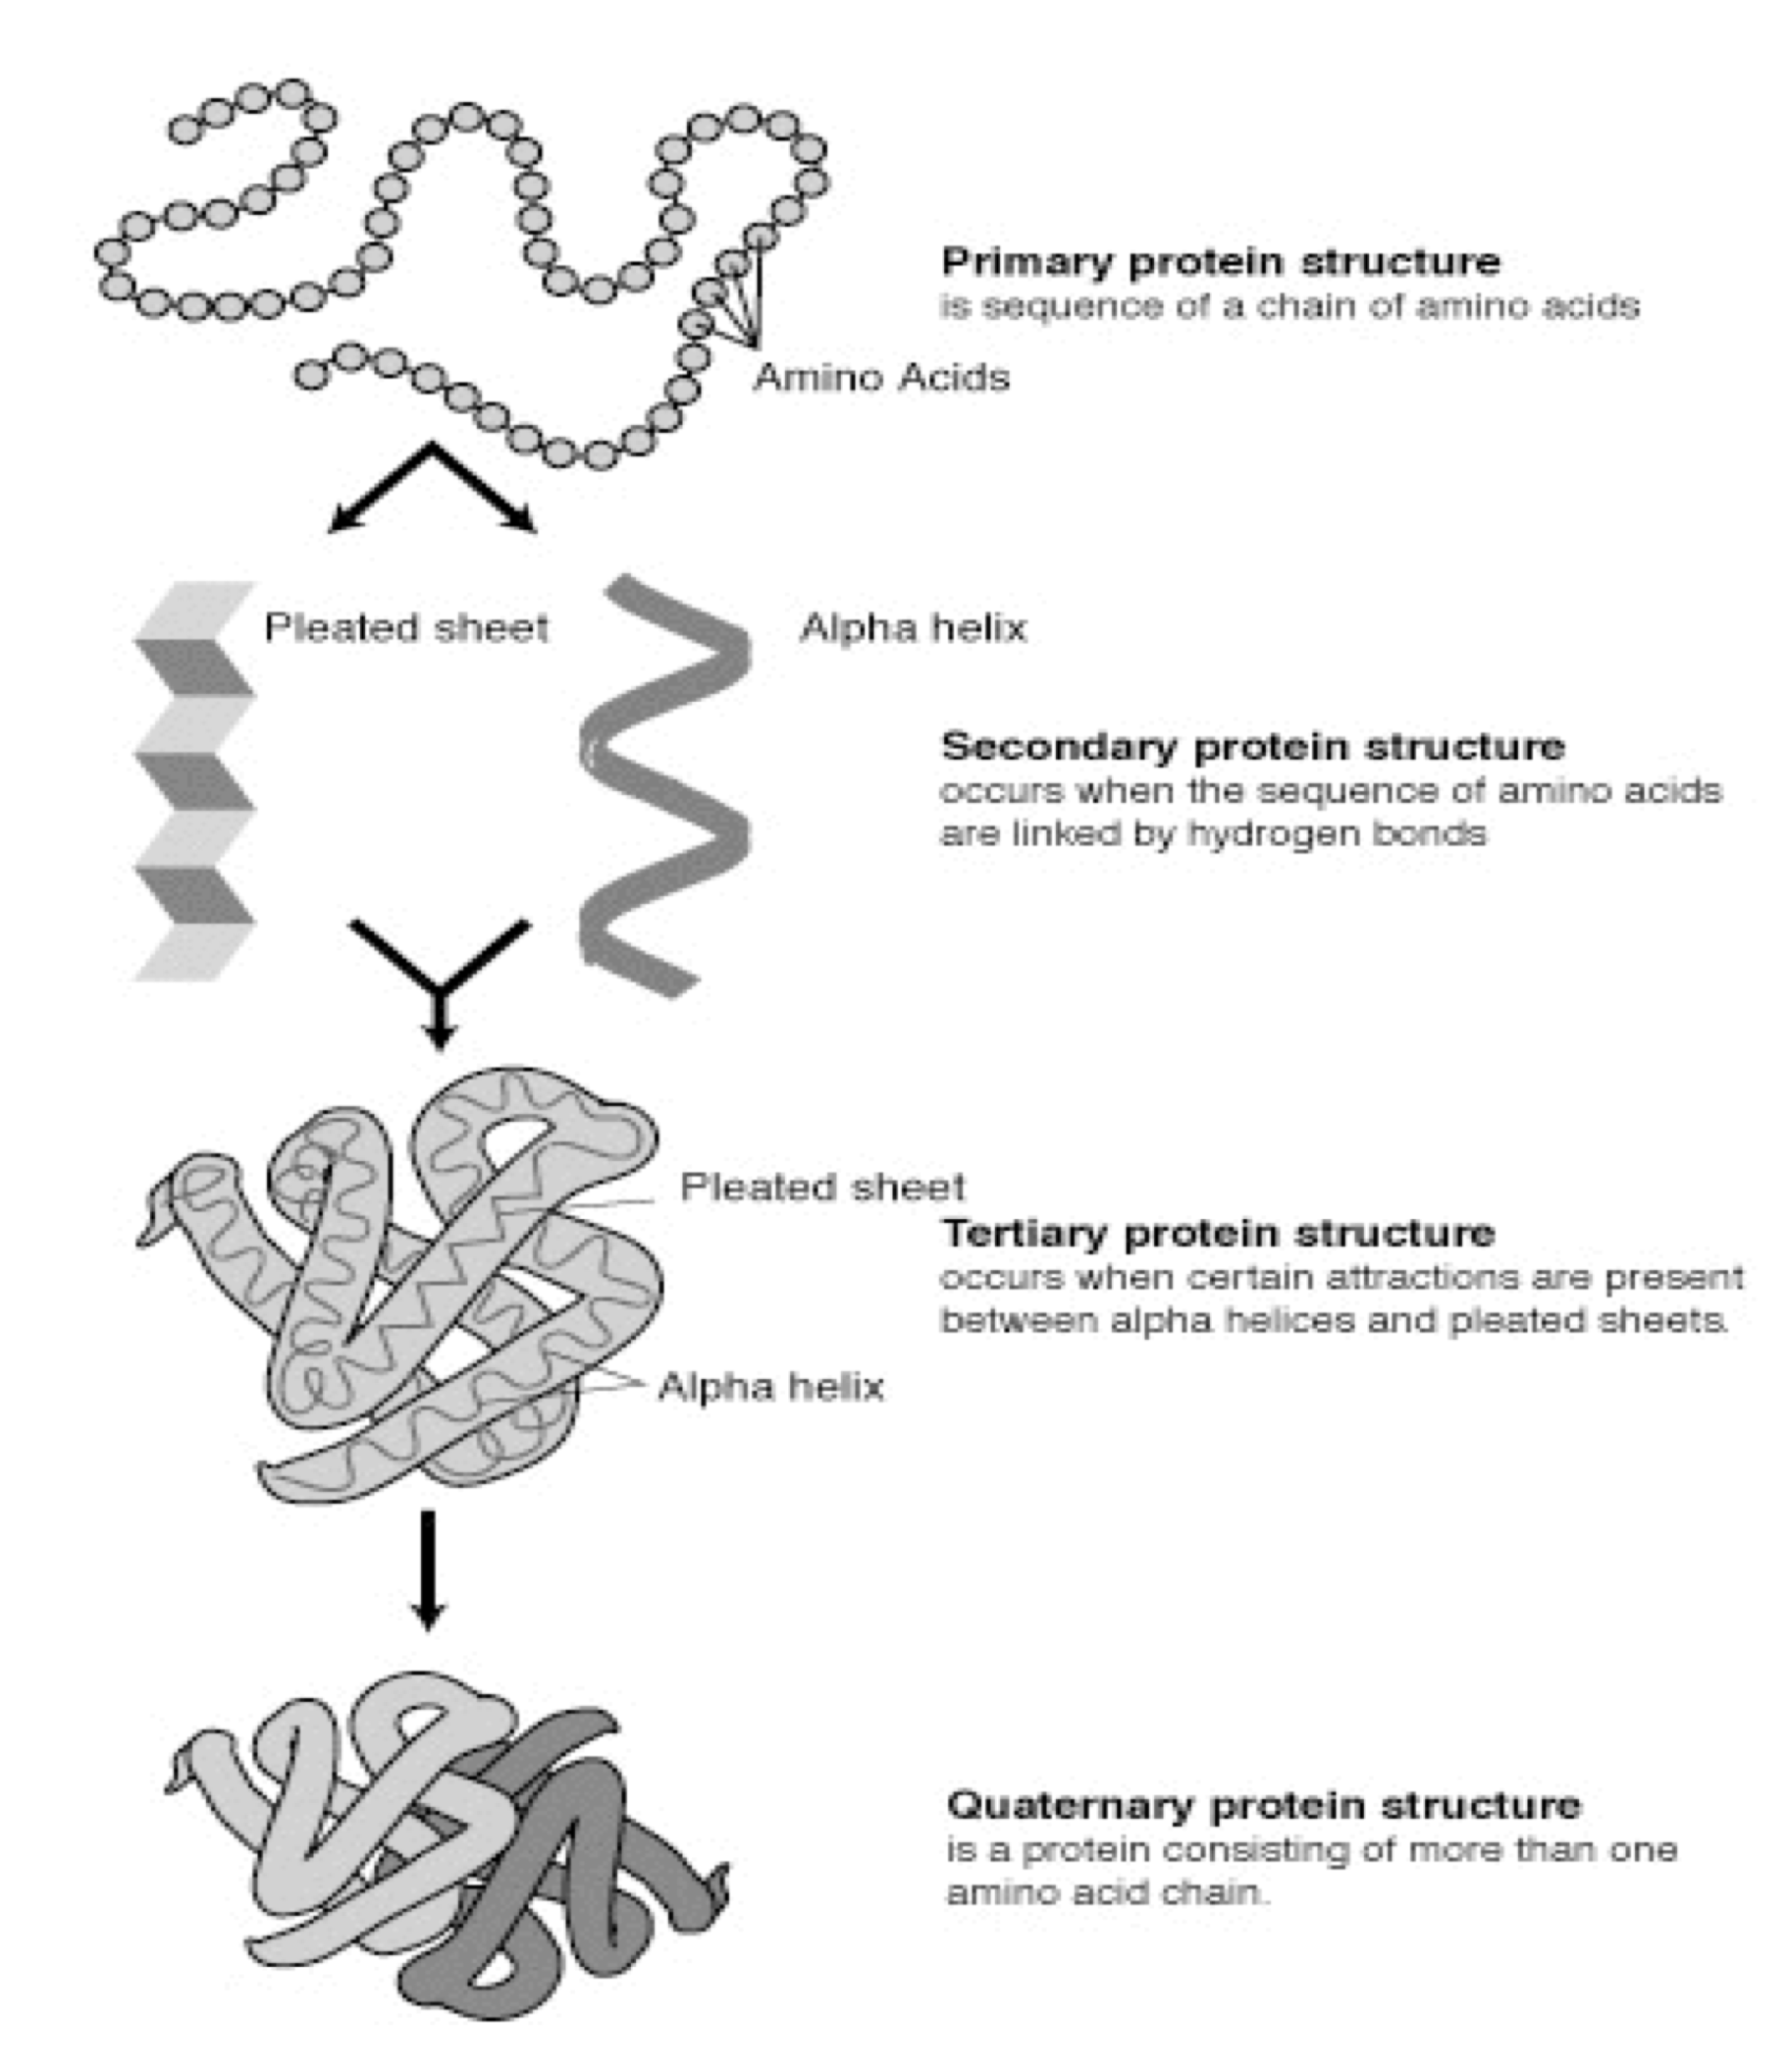
\includegraphics[width=0.5\textwidth]{figures/Proteine.png}
\end{center}
\paragraph{La struttura 3D di una proteina è molto complessa} La determinazione della
struttura 3D di proteine è un settore di ricerca molto attivo,
come mostra la crescita esponenziale di strutture depositate nel Protein Data Bank.\\
\section{Il cosmo "omico"}
\subsection{La genomica} 
\begin{itemize}
    \item \underline{Genoma:} Insieme dei geni di un organismo.
    \item \underline{Genomica:} scienza che se ne
    occupa.
    \item \underline{Genoma Umano:} Sequenziato
    completamente nel 2003.
    \item \underline{Occorre localizzare:} Elementi
    Funzionali:
    \subitem{-} Regioni 'utili' → geni;
    \subitem{-} Sequenze codificanti,
    comprendere i meccanismi che
    regolano l'espressione, scoprire
    la funzione, e cercare
    d'intervenire specificamente su
    quest'ultima.
\end{itemize}
Il costo del sequenziamento del genoma oggi è alla portata di ciascun individuo.
\subsection{Trascrittomica}
\begin{itemize}
    \item \underline{Trascrittoma:} l'insieme di tutti i
    trascritti (RNA messaggeri,
    mRNA)
    \item \underline{Trascrittomica:} scienza che se ne
    occupa.
    \item \underline{Occorre localizzare:} Profili di
    espressione:
    \subitem{-} più dinamico del genoma
    \subitem{-} microarrays monitorano i
    livelli di espressione di migliaia
    di geni allo stesso tempo.
    Mirano ad individuare
    correlazioni e legami tra
    espressione genica, attivazione
    e inibizione.
    Esempi: studio nella
    differenziazione di cellule
    staminali o evoluzione di
    tumori.
\end{itemize}
\subsection{Proteomica}
\begin{itemize}
    \item \underline{Proteoma:} l'insieme di tutte le
    proteine in un sistema biologico o
    nel suo genoma
    \item \underline{Proteomica:} scienza che se ne
    occupa.
    \item \underline{Occorre localizzare:} sia le
    proteine codificate dai geni che le
    possibili modificazioni post-
    traduzionali (gruppi prostetici,
    multidomini, fosforilazione, ecc).
    \item Alcune tecniche
    \subitem{-} Gel:
        \subsubitem 1° dimensione punto
        isoelettrico
        \subsubitem 2° massa molecolare
    \subitem{-} Spettrometria di massa:
    identifica una proteina in base
    al suo rapporto massa/carica in
    seguito a ionizzazione
\end{itemize}
\subsection{Genomica Strutturale}
\begin{itemize}
    \item \underline{Genomica strutturale:}
    determinazione della struttura
    terziaria e quaternaria (3D e
    domini) delle proteine.
    \item \underline{Tecniche:} cristallografia, NMR,
    homology modeling, cryoEM
    (microscopia crioelettronica)
    + AlphaFold (basato su AI)
    \item La struttura terziaria di una
    proteina è essenziale per
    determinarne la funzione
\end{itemize}
\subsection{Farmaco-genomica}
\begin{itemize}
    \item \underline{Farmacogenomica}: mira a
    prevedere la reazione di ciascun
    individuo verso un principio attivo
    in base al suo genotipo.
    \item \underline{Obiettivo:} creare terapie
    farmacologiche personalizzate
    per ottimizzare il risultato
    minimizzando gli effetti
    collaterali.
    \item Esempio: previsione di gravi
    reazione avverse a Abacavir
    nella terapia dell'HIV
\end{itemize}
\section{L'evoluzione ed il confronto tra sequenze}
Un allele (variante di un gene presente contemporaneamente
nella popolazione) può essere generato, fissato o mutare nel
tempo.\\
\textbf{Uno degli obiettivi in senso lato della bioinformatica è
stabilire se l'analisi dell'informazione riguardo a due
oggetti biologici (e.g. geni o proteine) permette di stabilire
una relazione di OMOLOGIA, cioè di discendenza da un
antenato comune}
Due sequenze che vengono separate fisicamente (per speciazione,
duplicazione ecc.) non si scambiano piu' "informazione" ed evolvono
indipendentemente, accumulando mutazioni. Spetta a noi trovare i tratti
conservati dal comune antenato.\\
Un modo per muoversi in tal direzione è allineare le sequenze e determinare la
percentuale di identita' o sequence identity (s.i.) (rapporto, in \% tra il numero
dei amminoacidi/basi identici rispetto al totale) o comunque il grado di similitudine.
Di norma, sequenze nucleotidiche non correlate hanno una s.i. ~50\%; sequenze
amminoacidiche non correlate hanno una s.i. ~20\%. Se tali valori aumentano,
aumenta la probabilità che le sequenze siano omologhe. Ma tale indice dovrebbe
tener conto anche della lunghezza delle sequenze.
Una s.i. del 90\% fra due sequenze di 100 a.a. ha un significato diverso rispetto alla
stessa s.i. su sequenze di 30 a.a.
\textbf{Allineare due sequenze significa stabilire se tra esse sussiste una
relazione di omologia}
\begin{titlepage}
    \begin{center}
        \vspace*{1cm}
        \LARGE
        \textbf{Lezione 2: Basi di Dati Biologiche}
        
    \end{center}
\end{titlepage}
\section{Le Basi di Dati Biologiche}
Il concetto di informazione è strettamente connesso a quello di dato e di
struttura.
Il dato è un osservabile (insieme di numeri, caratteri, simboli…)
La struttura è l' organizzazione ordinata di dati che ne consente
l'apprendimento.\\
Una banca dati è l'insieme di dati elementari, omogenei,
ordinati e fruibili. In altre parole: è una collezione
organizzata di dati
Esempio: elenco telefonico. L'informazione è strutturata in campi (nome,
cognome ecc.). Ogni persona con i propri dati è un record.
I dati biologici necessitano di un'organizzazione. Primo tentativo:
Margaret Dayhoff (1925-1983): raccolse, nel 1965, le sequenze di
65 proteine (lavoro pioneristico per il tempo!)
Le tecniche di sequenziamento rapido ed i progetti \textit{-omici} hanno
prodotto una quantita' esplosiva di dati, anche di sequenze
L'avvento di Internet ha facilitato di gran lunga l'acquisizione e la
distribuzione dell'informazione biologica in banche dati.\\
\subsection{Introduzione}
\begin{itemize}
    \item Sono collezioni di dati:
        \subitem{-} strutturati
        \subitem{-} indicizzati
        \subitem{-} aggiornati
        \subitem{-} interconnessi
    \item I database biologici sono legati a strumenti per:
        \subitem{-} recuperare records al loro interno 
        \subitem{-} aggiornare il database
        \subitem{-} combinare le informazioni
    \item Ci sono 6 principali categorie di basi di dati biologiche:
        \subitem{-} basi di dati di sequenze
            \subsubitem DNA
            \subsubitem RNA
            \subsubitem Proteine
        \subitem{-} basi di dati per il mapping
            \subsubitem geni
            \subsubitem cromosomi
            \subsubitem \dots
        \subitem{-} Strutture3d (PDB)
        \subitem{-} Trascrittomica
        \subitem{-} Funzionali (KEGG)
        \subitem{-} Per la letteratura (PubMed), ontologies (GO), \dots
\end{itemize}
A gennaio di ogni anno il Nucleic Accids Research pubblica un Database Issue, a gennaio:
\begin{itemize}
    \item nel 2020 contiene 89 nuovi database e l'aggiornamento di 90 database
    \item classificati nelle seguenti categorie
        \subitem{-} Nucleotide Sequence Databases
        \subitem{-} RNA sequence databases
        \subitem{-} Protein sequence databases
        \subitem{-} Structure Databases
        \subitem{-} Genomics Databases (non-vertebrate)
        \subitem{-} Metabolic and Signaling Pathways
        \subitem{-} Human and other Vertebrate Genomes
        \subitem{-} Human Genes and Diseases
        \subitem{-} Microarray Data and other Gene Expression Databases
        \subitem{-} Proteomics Resources
        \subitem{-} Other Molecular Biology Databases
        \subitem{-} Organelle databases
        \subitem{-} Plant databases
        \subitem{-} Immunological databases
        \subitem{-} Cell biology
        \subitem{-} COVID-19 databases
\end{itemize}
Le banche dati si strutturano e si integrano per favorire lo studio del dogma centrale della biologia.
Tre enti al mondo sono i principali.
\begin{itemize}
    \item EMBL
    \item NCBI
    \item DDBJ
\end{itemize}
Integrando collegamenti esterni (Swiss-prot, ExPASy,
UCSC, ecc, ecc…) sono un punto ideale di partenza.
\subsection{Dati di Sequenza}
Che dati si possono trovare?
\begin{itemize}
    \item Principalmente sono presenti
        \subitem{-} sequenze di caratteri (nucleotidi, amminoacidi)
        \subitem{-} o strutture
    \item L'uso della rappresentazione dei dati biologici di
    varia natura come sequenze è la forma di gran lunga
    più diffusa.
    \item Sequenze di DNA: formate da 4 tipi di lettere (a,c,g,t), convenzionalmente minuscole
    \item Sequenze di RNA: formate da 4 tipi di lettere (A,C,G,U), convenzionalmente maiuscole
    \item Sequenze proteiche: formate da 20 lettere (A, C, D, E, F, G, H, I,K, L, M, N, P, Q, R, S, T, V, W, Y), convenzionalmente maiuscole
\end{itemize}
Il formato FASTA-Pearrson: 
\begin{itemize}
    \item Rappresentazione mediante testo di sequenze nucleotidiche o
    peptidiche (lettere MAIUSCOLE).
    \item La prima riga (di lunghezza arbitraria) è preceduta da ">" e rappresenta
    la descrizione della sequenza.
    \item Le linee precedute da ">" o ";" sono considerate di commento e non
    vengono interpretate come dato di sequenza
    \item Le linee successive (ciascuna di 80 caratteri) rappresentano la
    sequenza.
    \item Un file fasta può avere estensione (non c'è uno standard)
\end{itemize}
Il formato XML (eXtensible Markup Language).
\begin{itemize}
    \item Replica la struttura logica del record nella banca dati
    \item I tag permettono di delimitare e definire campi e sottocampi
\end{itemize}

\section{NCBI}
NCBI (National Center for Biotechnology Information) presso il National Institute of Health. Offre accesso a tante risorse di vario tipo:
\begin{itemize}
    \item Sequenze geniche e proteiche
    \item Strutture terziarie
    \item Genomi completi
    \item Pathways
    \item EST (expressed sequence tags)
    \item Profili trascrittomici
    \item Cataloghi tassonomici
\end{itemize}
Fornisce accesso a numerosi database attraverso il sistema Entrez:
\begin{itemize}
    \item GenBank
    \item Swissprot
    \item PubMed
    \item GEO 
    \item \dots
\end{itemize}
Fornisce accesso anche a diversi software bioinformatici.
\subsection{Com'è strutturato il database}
Una ricerca qualunque dall'home page apre ENTREZ,
interfaccia per l'accesso ai database presenti in NCBI.\\
\begin{itemize}
    \item PubMed è l'interfaccia di accesso a
    MEDLINE.
    Con I suoi
    \subitem{-} 20 milioni di record fino agli anni '50
    \subitem{-} 4600 riviste da più di 70 paesi\\
    È la banca dati per la letteratura
    biomedica più completa.
    (Accessibile anche tramite EBI tramite 17 CiteXplore)
    \item Nucleotide è un database che
    raccoglie sequenze da diversi altri
    database di NCBI.
    Per sequenze nucleotidiche
    \subitem{-} EST ( expressed sequence tag )
    \subitem{-} GSS ( genome sequence surveys
    Gene è orientato ai geni, ai loci
    altre sequenze, B act A rtif C hromosome ,
    Y east A rtif C hromosome ,\dots)\\
    Inoltre:
    \subitem{-} RefSeq ( sistema di
    identificazione )
    \subitem{-} Unigene ( sequenze raggruppate )
    \subitem{-} UniProt ( proteine )
    \item Gene è orientato ai geni, ai loci
    \item Proteins è la sezione focalizzata sulle
    proteine, alle quali possono
    corrispondere strutture
    \item PubChem dedicato ai composti chimici
    \item In Genome genomi completi con riferimenti alla
    ricerca effettuata, varianti genomiche,
    ecc
    \item Informazioni su profili di espressione
    genica in diverse condizioni, modifiche
    post-traduzionali
    GEO (Gene Expression Omnibus)
    repository
\end{itemize}
GenBank è la banca dati di tutte le sequenze in NCBI (sincronizzata con
EMBL e DDBJ). Le sequenze derivano da diverse fonti e tipi:
\begin{itemize}
    \item Geni (regioni di regolazione, esoni, introni: unità ereditarie)
    \item EST (Expressed Sequence Tags)
    brevi segmenti di DNA trascritti e sequenz. da cDNA (ottenuto da
    mRNA retrotrascritto)
    \item STS (sequence tagged site, dove l'informazione genetica è mappata
    fisicamente)
    \item GSS (Genome Survey Sequence, vettori sequenze solo parzialmente sequenziate)
    \item HTGS (High Throughput Genomic Sequence, sequenze prodotte da tecniche di
    seconda generazione per il sequenziamento veloce, messe qui in “preview”)
    \item Sequenze di proteine (sezione nr, non redundant)
\end{itemize}
Così tanto materiale ha provocato l'esigenza di ordine: \textbf{RefSeq}.\\
RefSeq è stato ideato per far corrispondere a ciascun trascritto
normalmente prodotto da un gene e a ciascuna proteina una sequenza di
riferimento, un identificatore (accession number).\\
Altri esempi di identificatori NON RefSeq sono:
\begin{itemize}
    \item X02775 GenBank/EMBL/DDBJ nucleotidic sequence
    \item Rs7079946 dbSNP (single nucleotide polymorphism)
    \item N91759.1 An expressed sequence tag
    \item AAC02945 GenBank protein
    \item Q28369 SwissProt protein
    \item 1KT7 Protein Data Bank structure record
\end{itemize}
Refseq fornisce un identificatore per la sequenza di riferimento, curato dal
personale dell'NCBI.\\
formati principali degli id RefSeq sono:
\begin{itemize}
    \item Complete genome/chromosome/plasmid N\textbf{C}$\_\#\#\#\#\#\#$
    \item Genomic contig (segmenti sovrapposti di DNA segments che rappresentano una sequenza consenso) N\textbf{T}$\_\#\#\#\#\#\#$
    \item mRNA (DNA format) N\textbf{M}$\_\#\#\#\#\#\#$
    \item Protein N\textbf{P}$\_\#\#\#\#\#\#$
\end{itemize}
\paragraph{Un primo esempio di ricerca - L'Emoglobina}
Una delle prime proteine ad essere studiata (anni '30 e '40, da Mulder, Liebing et al.).\\
È stata la prima proteina ad essere usata negli allineamenti multipli di sequenza:
voglio fare dei confronti di sequenze (ad esempio per confrontare la stessa proteina prodotta da diverse specie). Con le prime tecniche di sequenziamento abbiamo scoperto che è stata localizzata in due loci, uno sul cromosoma 16 (subunità alfa) e 11 (subunità beta). I due geni sono regolati sia in base all'età che in base ai diversi tessuti.\\
È quindi un problema complesso che ha poi originato una serie di considerazioni.
La mioglobina, una globina (struttura globulare a 8 eliche)
che lega l'ossigeno nei tessuti muscolari, è stata la prima
proteina la cui struttura tridimensionale è stata risolta
tramite cristallografia.\\
L'emoglobina è un tetramero (due catene alfa e due beta negli
adulti) è il principale trasportatore di ossigeno nei vertebrati.
Assieme alla mioglobina è stata usata nei primi studi sugli
allineamenti multipli.\\
Negli anni '80 con le prime tecniche di sequenziamento è stata
localizzata in due loci, uno sul cromosoma 16 (subunità alfa) e 11
(subunità beta). I due geni sono regolati sia in base all'età che in
base ai diversi tessuti.
\subsubsection*{Ricerca dell'emoglobina}
\begin{enumerate}
    \item Inseriamo "beta globin" nella barra di ricerca
    \item Seguiamo poi il link a "Gene"
    \item Entrez Gene (ex LocusLink) è un portale curato che descrive loci genetici
        \subitem{-} nomenclatura
        \subitem{-} alias
        \subitem{-} accession numbers
        \subitem{-} fenotipi
        \subitem{-} OMIM (ereditarietà dei caratteri)
        \subitem{-} HomoloGene
        \subitem{-} mappatura sul genoma
        \subitem{-} collegamenti esterni
    \item In generale ad oggi quesa ricerca trova 126 entries
    \item Intestazione: Entrez Gene, Noa: "Official Symbol", HBB per la beta globina
    \item Limitiamoci alla ricerca per Homo Sapiens (selezionando sulla destra da Results by taxon)
    \item Cliccando la specie si aggiorna automaticmente la stringa di ricerca: {\ttfamily(beta globin) AND "Homo sapiens" [ porgn:\_txid9606 ]}
    \item Con il limite Homo Sapiend le entries sono solo 41
    \item Apriamo la prima entry
    \item Sulla dx in basso troviamo numerosi link a database esterni
    \item Abbiamo una sezione sulle regioni genomiche, una sulla bibliografia
    \item Sezione interessante: GeneRif (intended to facilitate access to publications documenting experiments that add to our understanding of a gene and its function)
    \item E ancora Fenotipi, Variazione Genica, Pathways per Biosistemi e Interazioni note con altri geni.
    \item Ontologia: (fondamentale per sistemi automatici di apprendimento). Classificazione
    e organizzazione dei dati in categorie predefinite così da agevolare l'individuazione di
    analogie e caratteristiche primarie. Può essere di diversi tipi, ma la principale distingue:
        \subitem{-} Funzione molecolare
        \subitem{-} Localizzazione cellulare
        \subitem{-} Processo biologico
    \item Catalogazione RefSeq (a fine pagina)
\end{enumerate}
\subsection{Operatori Booleani}
\subsubsection{Operatore AND (\&)}
Restringe il campo di ricerca, inserendo ad es. la stringa:
{\ttfamily equus caballus AND hemoglobin alpha}\\
La banca dati ci mostrerà una lista di sequenze proteiche i cui campi di
descrizione contengono entrambe le parole. Quindi le sequenze proteiche
del cavallo che non contengono nella descrizione la parola hemoglobin
non vengono selezionate.
\subsubsection{Operatore OR (|)}
Estende il campo di ricerca, digitando ad esempio:
Restringe il campo di ricerca, inserendo:
{\ttfamily homo sapiens OR mus musculus}\\
Otterremo una lista di sequenze i cui campi contengono la parola homo
sapiens o la parola mus musculus.
L'operatore allarga l'insieme
delle sequenze che incontrano le nostre esigenze.
\subsubsection{Operatore NOT (!)}
Restringe il campo di ricerca, inserendo:
{\ttfamily homo sapiens NOT hemoglobin}
Richiederemo sequenze i cui campi contengono la parola homo sapiens
ma non la parola hemoglobin.
\subsubsection{Combinazione di Operatori Booleani}
Gli operatori booleani si possono combinare, vengono letti da sinistra a
destra. Per questo sono utili le parentesi. Ad esempio: globin AND promoter OR enhancer produce quasi 5000
hits. Ma se si scrive globin AND (promoter OR enhancer) se ne
ottengono circa 70.\\
Altre possibilità sono:
\begin{itemize}
    \item Specificare un organismo (human, nella query:
    human[ORGN]
    \item Usare l'asterisco: glob * restituisce tutte le entry che
    contengono una stringa che inizia per “glob”
    \item Usare le virgolette “” . La ricerca di “toxin B1” restituirà le
    entries che contengono esattamente la stringa intera.
    \item \dots
\end{itemize}
\subsection{Nel dettaglio}
\paragraph{Homologene}
la risorsa ideale per individuare gruppi
di geni omologhi negli eucarioti presenti in NCBI
\paragraph{OMIM}
Catalogo di geni umani e disordini genetici
\paragraph{SNP}
Single Nucleotide Polimorfism
\newpage
\section{Proteine - Le banche dati proteiche più usate}
\paragraph{Uniprot}
(Universal Protein Resource) raccoglie le informazioni dei database:
\begin{enumerate}
    \item Swiss-prot (SIB)
    \item TrEMBL (EBI) 
    \item PIR
\end{enumerate} 
Offre la possibilità di effettuare Text
Search o Blast Search. Viene curato anche un database NON RIDONDANTE
(UniRef).
\paragraph{Swissprot}
Molto curato e detagliato, con annotazioni circa funzione, struttura, modificazione e altre informazioni utili.
\paragraph{TrEMBL}
È la traduzione in silico di ogni entry codificante del database primario dell'EMBL, non è accurato, ma è ricchissimo.
\paragraph{PIR}
È il discendente diretto del database della Dayhoff, è curato a mano e le annotazioni sono molto ricche e precise.
\subsection{NCBI Protein - non molto ricco}
Entrez Protein: Contiene diverse informazioni su proteine
\begin{itemize}
    \item 147 amminoacidi
    \item PRI: primates
    \item $NP\_000509$ (protein accession number)
    \item $NM\_000518.4$ (mRNA, RefSeq)
    \item Riferimenti bibliografici
    \item Sequenze FASTA (Opzione Display)
    \item Siti di modificazione post-traduzionale (AA94, AA121)
    \item Riferimenti ad altri database
    \item Sequenza amminoacidica (1 lettera)
\end{itemize}
È un record non molto ricco dal punto di vista dei dati delle proteine.
\subsection{Uniprot}
Uniprot è il più completo database centralizzato per le sequenze proteiche.\\
È organizzato su 3 livelli:
\begin{enumerate}
    \item Uniprot Knowledge Base
        \subitem{-} Swiss-Prot (curato)
        \subitem{-} TrEMBL (automatico)
    \item UniProt Reference
    clusters (UniRef)
        \subitem{-} Cluster di proteine che
        condividono il 50\%, 90\%,
        100\% di identità di
        sequenza
    \item UniProt Archive (UniParc)
        \subitem{-} Archivio di sequenze
        proteiche stabile, non
        ridondante, da diverse 58 fonti
\end{enumerate}
\subsubsection{Struttura del database}
Nella homepage abbiamo la classica barra di ricerca e subito sotto i link di accesso alle diverse informazioni contenute in Uniprot.\\
\paragraph{Un esempio di ricerca}
\begin{enumerate}
    \item Inseriamo "{\ttfamily hbb}" nella barra di ricerca.
    \item Sulla sinistra possiamo selezionare gli organismi a cui restringere la ricerca. Selezioniamo Humans.
    \item Questo aggiornerà automaticamente la stringa di ricerca: {\ttfamily hbb AND organism: "Homo sapiens (Human) [9605]"}
    \item Selezioniamo la prima entry.
    \item Sulla sinistra troviamo la tavola con tutti i contenuti disponibili.
    \item Tra i più importanti abbiamo: "Function" (che specifica la funzione della proteina), "Pathology \& Biotech", "Expression", "Interaction", "Family \& Domains", \dots
    \item In "Structure" e altre sezioni troviamo i link a PDB (Protein Data Bank), database di strutture proteiche.
    \item In "Sequence" troviamo tutta la sequenza proteica, scaricabile in formato FASTA.
    \item Abbiamo inoltre vari link di collegamento ad altri database di sequenze (EMBL,GeneBank, DDBJ), varianti, \dots
\end{enumerate}
\subsection{ExPASy}
(Expert Protein Analysis System)\\
È una risorsa curata, espressione del SIB (Swiss Institute of
Bioinformatics). Principalmente dedicata alle proteine.\\
La risorsa principale che ha prodotto è SwissProt (confluita in Uniprot). Rimane un punto di riferimento per molti tools. 

\begin{titlepage}
    \begin{center}
        \vspace*{1cm}
        \LARGE
        \textbf{Lezione 3: Allineamenti di Sequenze - concetti e algoritmi}

    \end{center}
\end{titlepage}
\section{Allineamenti di Sequenze}
Un primo e precoce allineamento di sequenze si ha nel 1961: H.C. Watson and J.C. Kendrew,
“Comparison Between the Amino-Acid Sequences of Sperm Whale Myoglobin and of Human Hæmoglobin.” Nature 190:670-672, 1961.\\
\paragraph{L'allineamento di sequenze a coppie è un'operazione fondamentale in bioinformatica}
È utilizzato per decidere se due proteine (o geni) sono correlate strutturalmente e funzionalmente.\\
Viene utilizzato per identificare i domini o motivi che sono
condivisi tra le proteine. È alla base della ricerca con BLAST (prossime lezioni) e viene utilizzato anche per l'analisi dei genomi.
\paragraph{Allineamento a coppie: sequenze di proteine possono essere più informative del DNA}
Le proteine sono più informative del DNA (20 vs 4 caratteri);
molti aminoacidi condividono proprietà biofisiche.\\
Ricordiamo che i codoni sono degenerati: i cambiamenti in terza posizione
spesso non alterano l'amminoacido che ne è specificato
(mutazioni sinonime). Le sequenze di proteine offrono un più lungo tempo di
"look-back" e le sequenze di DNA possono essere tradotte in proteine,
e poi utilizzate negli allineamenti a coppie.
\subsection{Definizione - \underline{Allineamento a coppie}}
Il processo che allinea due sequenze per
raggiungere livelli massimi di identità (e
conservazione, nel caso di sequenze di
amminoacidi) al fine di valutare il grado di
similitudine e la possibilità di omologia.
\subsection{Altre definizioni}
\begin{itemize}
    \item \underline{\textbf{Identità}}
        \subitem La misura in cui due sequenze (di nucleotidi o aminoacidi) sono
        invarianti. (es. identità del 32\% => 32 a.a. su 100 sono
        ordinatamente identici)
    \item \underline{\textbf{Conservazione}}
        \subitem In una sequenza, modifiche in una specifica posizione di un
        amminoacido (o meno comunemente, di un nucleotide) che
        preservano le proprietà fisico-chimiche del residuo originale.
    \item \underline{\textbf{Similitudine}}
        \subitem La misura in cui due sequenze (di nucleotidi o aminoacidi)
        sono correlate. Si basa su identità + conservazione.
    \item \underline{\textbf{Omologia}}
        \subitem Similitudine attribuita a discendenti da un
        antenato comune.
        \subitem{!} \textbf{Nota bene:}
            \subsubitem{-} OMOLOGIA indica che due entità (es. 2 sequenze) hanno
            una stessa origine filogenetica, cioè derivano da un antenato
            comune. È un carattere QUALITATIVO.
            \subsubitem{-} SIMILITUDINE indica che due entità (es. 2 sequenze), in
            relazione ad un certo criterio comparativo, hanno un certo
            grado di similitudine. È un carattere QUANTITATIVO
            (vedremo tra breve come definirla).
        \subitem{!} \textbf{Osservazioni:}
            \subsubitem{-} La struttura di una proteina dipende della sua sequenza di a.a. (concetto alla
            base del Protein Folding).
            \subsubitem{-} La struttura determina la funzione molecolare della proteina.
            \subsubitem{-} Se una sequenza proteica è conservata durante l'evoluzione ed è quindi
            presente in organismi diversi (famiglia di proteine) è ragionevole assumere che le
            funzioni che svolge siano simili o per lo meno correlate.
        \subitem{!} \textbf{Passi per predizione di funzione:}
            \begin{enumerate}
                \item Identificazione delle proteine di una famiglia (evolute da un
                progenitore comune $\rightarrow$ sequenza di a.a. abbastanza simile.)
                \item dentificazione degli a.a. che svolgono un ruolo strutturale o
                funzionale analogo (allineamento).
            \end{enumerate}
\end{itemize}
\paragraph{Esempio 1:} la catena $\beta$ dell'emoglobina e miogobina «si somigliano» 
\begin{center}
    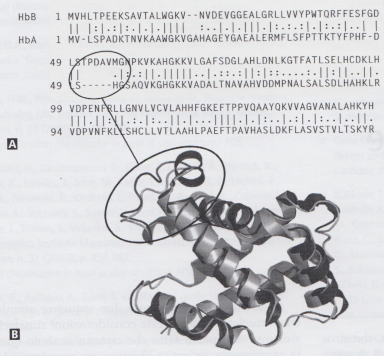
\includegraphics[width=0.5\textwidth]{figures/globine.png}
    \captionof{figure}{Le zone con indel nelle sequenze sono strutturalmente dissimili}
\end{center}
\begin{itemize}
    \item \underline{\textbf{Ortologhi}}
        \subitem Sequenze omologhe in diverse specie che derivano,
        tramite la speciazione, da un gene ancestrale
        comune. La funzione può essere o non essere
        simile.
    \item \underline{\textbf{Paraloghi}}
        \subitem Sequenze omologhe all'interno di una singola specie
        sorte dalla duplicazione genica.
\end{itemize}
\begin{center}
    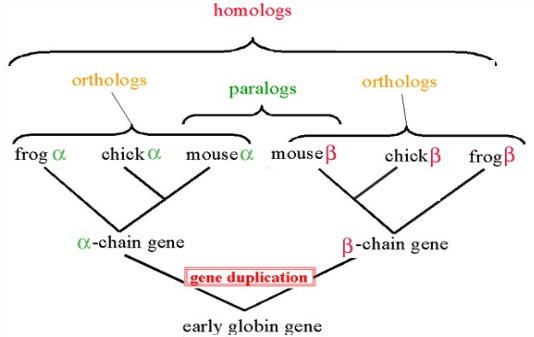
\includegraphics[width=0.5\textwidth]{figures/ortpar.png}
    \captionof{figure}{Ortologhi e paraloghi sono spesso rappresentati in un albero singolo.}
\end{center}
\newpage
Ortologhi: membri di una famiglia di geni (proteine) in vari organismi.
\begin{center}
    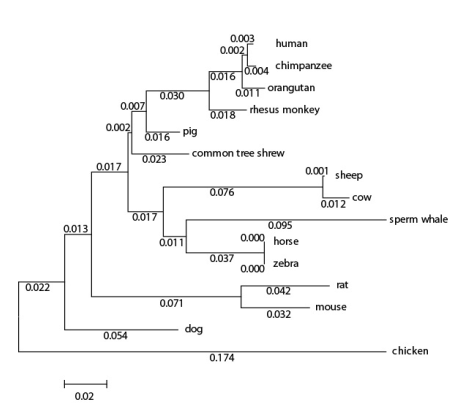
\includegraphics[width=0.5\textwidth]{figures/ortpar2.png}
    \captionof{figure}{Questo albero mostra gli ortologhi della globina.}
\end{center}
Paraloghi: i membri di una famiglia di geni (proteine) all'interno di una specie.
\begin{center}
    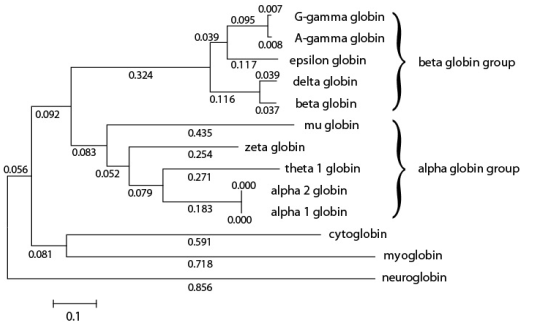
\includegraphics[width=0.5\textwidth]{figures/ortpar3.png}
    \captionof{figure}{Questo albero mostra i paraloghi della globina umana.}
\end{center}
\section{Confrontare due sequenze}
\paragraph{Come posso trasformare una stringa in un'altra?} 
Un modo semplice per capirlo è allineare le due stringhe:\\
ESEMPIO: 1 - LA CASA NUOVA; 2 - LA CASSA VUOTA\\
\begin{center}
    1 - L A C A - S A N U O V A\\
    2 - L A C A S S A V U O T A\\
    oppure\\
    1 - L A C A - S A - N U O V A\\
    2 - L A C A S S A V - U O T A\\
\end{center}
Nel secondo caso c'è un'operazione in più. 
\begin{itemize}
    \item Il numero minimo di operazioni necessarie per allineare
    due sequenze ne misura la distanza.
    \item La Natura dispone di varie operazioni per trasformare un
    oggetto nell'altro (mutazioni, indel…)
    \item L'evoluzione sceglie la via piu' breve (principio di
    massima parsimonia); cio' si manifesta tramite l'analisi
    dell'allineamento.
\end{itemize}
Dobbiamo avere chiari i concetti di match (residui
appaiati), mismatch (sostituzioni) e gap (indel).
\subsection{Come identificare le zone di somiglianza locale tra due sequenze?}
\subsubsection{Matrice a punti - dot plot}
È un modo relativamente semplice.\\
Confrontiamo la stringa con se stessa (autoconfronto):
\begin{enumerate}
    \item Mettiamo una x per ogni identità
\end{enumerate}
\begin{center}
    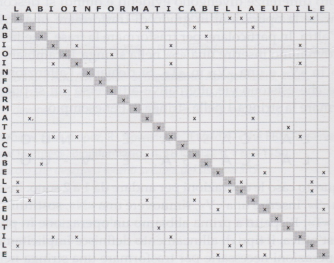
\includegraphics[width=0.5\textwidth]{figures/autoconfronto.png}
    \captionof{figure}{\dots piuttosto banale. Cambiamo la seconda stringa.}
\end{center}
Effettuiamo un'inversione. Il pattern delle diagonali lo
mostra chiaramente: la diagonale principale si spezza ma
porzioni delle stringhe sono identiche.
\begin{center}
    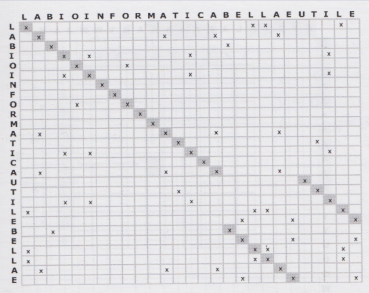
\includegraphics[width=0.5\textwidth]{figures/inversione.png}
\end{center}
Possiamo individuare facilmente alcuni patterns mediante le matrici a punti (la prima stringa in alto resta immutata):
\begin{itemize}
    \item Inversione di parole\\
    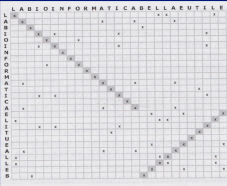
\includegraphics[width=0.3\textwidth]{figures/inv2.png}
    \item Ripetizione di parole\\
    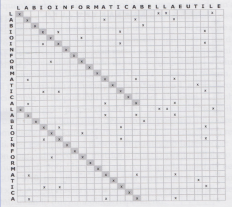
\includegraphics[width=0.3\textwidth]{figures/rip.png}
    \item Delezione di caratteri\\
    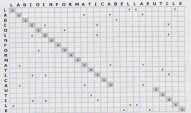
\includegraphics[width=0.3\textwidth]{figures/del.png}
\end{itemize}
Se però allineamo sequenze di acidi nucleici (solo 4 lettere) il “segnale” di similitudine è mascherato dal grande rumore di fondo. Servono FILTRI per ridurre il rumore.
\paragraph{Una semplice osservazione:}le zone delle sequenze più simili
localmente si distribuiscono su diagonali; le altre somiglianze puntiformi si distribuiscono casualmente.
Allora, è meglio confrontare le sequenze non per singole posizioni, ma per interi segmenti (FINESTRE).\\
Potremmo usare delle finestre scorrevoli.\\
ESEMPIO: confrontiamo una finestra di 5 residui in una seq
con una finestra di 5 residui nell'altra. Confronto tutte le
finestre (facendole scorrere), e metto una * al centro della
finestra solo se ho un match totale.
\begin{center}
    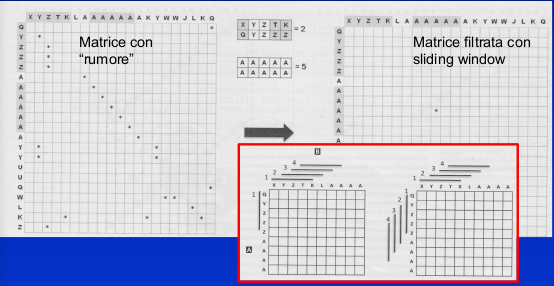
\includegraphics[width=0.5\textwidth]{figures/sliding.png}
\end{center}
In generale: si fa scorrere una finestra alla volta.
\paragraph{La procedura}
\begin{enumerate}
    \item Definiamo la posizione di una casella $(x,y)$.
    \item Fissiamo il centro della finestra, di raggio $g$.
    \item La lunghezza della finestra è dunque: $L= 2g+1$
    \item Il numero $N$ di residui identici in quella finestra è allora: $N(x,y) = \sum^{+g}_{h=-g} S(x + h, y+h)$
        \subitem $S=1$ se il carattere in $x+h$ è identico a quello in $y+h$; altrimenti $S=0$
\end{enumerate}
Questa regola è però molto restrittiva. A noi interessa anche
la similitudine, non solo l'identità. Potremmo definire una soglia $s$, per cui:
\begin{itemize}
    \item Se $N(x,y)>s$ mette un simbolo nella casella in posizione $x,y$.
\end{itemize}
Dobbiamo quindi misurare la similitudine, e.g. tra aa o basi. Un
esempio di matrice di punteggio (non di punti!!) per seq
di nucleotidi può essere:
\begin{center}
    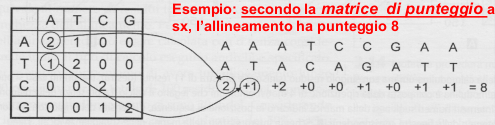
\includegraphics[width=0.5\textwidth]{figures/mat.png}
\end{center}
Misurata la similitudine, possiamo allora attribuire un nuovo punteggio al confronto fra due finestre:
\begin{itemize}
    \item Se $N(x,y)$ è il numero dei residui simili, ed è la media dei punteggi
    delle singole coppie prelevati dalla matrice di punteggio scelta:
    \item $N(x,y) = \sum^{+g}_{h=-g} {S(x + h, y+h)\over L}$
\end{itemize}
$S$ ora dipende da quale matrice di punteggio scegliamo e dalla
lunghezza della finestra. Possiamo quindi essere un po' più "elastici" pur mantenendo
la regola:
\begin{itemize}
    \item Se $N(x,y)>s$ mette un simbolo nella casella in posizione $x,y$.
\end{itemize}
$s$ lo decide la matrice di punteggio (cioè la similitudine).
\subsubsection{In breve}
In conclusione, la visualizzazione (ed il calcolo) di una
matrice a punti dipende da:
\begin{enumerate}
    \item La lunghezza $L$ della finestra scorrevole scelta
    \item Il metodo per misurare la similitudine $S(x,y)$
    \item La soglia $s$ per “marcare” la casella rispettiva
\end{enumerate}
In pratica conviene fissare 2 parametri e variare il terzo per rendere le zone di
similitudine più evidenti. Molti programmi fanno questo.\\
Es. DOTTER/Dotlet - assegna un colore dipendentemente da $S$.
\paragraph{Nota:}Analogamente all'identità di sequenza, che si può
misurare in percentuale (\%), anche la similitudine, una volta
quantificata, si può misurare in \%.\\
$S_1$ e $S_2$ sono due sequenze lunghe, rispettivamente, $L_1$ ed $L_2$.\\
Scelta $L_1$ come riferimento si ha:
$$ SequenceIdentity(s.i.) = ({\#matches \over L_1}) * 100 $$
$$ SequenceSimilarity(s.s.) = ({S_1 vs. S_2 s.c. \over S_1 vs. S_2 i.c.}) * 100 $$
\textit{s.c. = similarity score, ed è ottenuto allineando $S_1$ con $S_2$, e attribuendo il punteggio ottenuto dalla matrice discore.\\i.c. = identity score ed è ottenuto allineando $S_1$ con sè stessa ed attribuendo il punteggio ottenuto dalla matrice di score}
\textit{\\Nota:} se sono presenti indel, a denominatore metto la lunghezza
dell'allineamento (compresi gli indel), e non la lunghezza originale della sequenza.
\section{Algoritmi dinamici di allineamento}
I dot plots non tengono in considerazione gli indel. Occorrono altri
algoritmi che, passo a passo e seguendo una certa direzione, trovino
l'allineamento con:
\begin{itemize}
    \item Maggior numero di simboli identici
    \item Minor numero di indel (sfavorite evolutivamente)
\end{itemize}
Esempio: proviamo tutte le combinazioni da sx a dx, riempiendo una colonna alla volta (qui mostriamo solo i primi 3 residui!!)\\
Stabiliamo inoltre i punteggi:
\begin{itemize}
    \item -1 per indel
    \item 0 per residui diversi
    \item +1 per residui identici
\end{itemize}
Il numero delle combinazioni possibili è molto grande, specie per
sequenze lunghe. Nel 1970 NEEDLEMAN e WUNSCH creano un algoritmo, poi
migliorato ed esteso. Noi analizziamo l'originale.
\subsection{Il concetto}
distribuiamo le due sequenze in una matrice. Il possibile
allineamento tra le due identifica un percorso che unisce le caselle dei
residui appaiati.
\begin{center}
    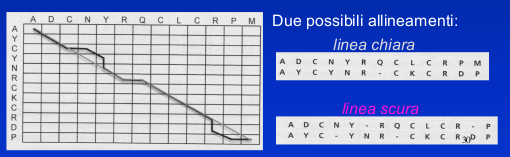
\includegraphics[width=0.5\textwidth]{figures/algo.png}
\end{center}
\subsection{Regole pratiche}
\begin{enumerate}
    \item Il percorso ha una direzione e procede solo in avanti (NON si torna indietro!)
    \item Occorre trovare il percorso con il \textbf{maggior} numero di aa identici e il \textbf{minor} numero di indel
    \item Occorre anche tener conto della similitudine fra amminoacidi (significato evolutivo)
    \item IMPORTANTE: un allineamento ottimale è sempre
    composto da suballineamenti ottimali (cioè: togliendo uno
    ad uno i residui dal fondo, l'allineamento deve restare
    ottimale, per poter ricostruire il percorso a ritroso)
\end{enumerate}
\subsection{Step}
\begin{enumerate}
    \item INIZIALIZZAZIONE della matrice: regola molto semplice; 1
    se identici, 0 altrimenti. N.B. ora $(x,y)$ identifica: (residuo in
    colonna, residuo in riga) (N.B. dopo aver trattato le matrici
    di score potremo normalizzare diversamente)\\
    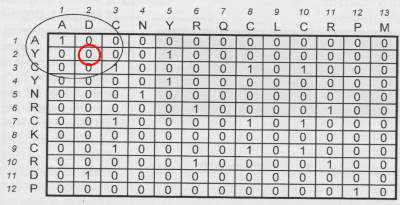
\includegraphics[width=0.6\textwidth]{figures/init.png}
    \item Partiamo da (1,1) (in alto a sx:
    la direzione è importante!!):
    (1,1) $\rightarrow$ (2,2)
    L'unico percorso possibile è
    questo: per “ricordarmelo”
    sommo il valore della cella
    (1,1) a quello della cella (2,2)
    da matrice inizializzata
    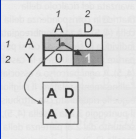
\includegraphics[width=0.3\textwidth]{figures/due.png}
    \item Prossimo step: verso (2,3). Ci sono due possibili percorsi, corrispondenti a due diversi
    allineamenti: scelgo quello con punteggio finale maggiore, sempre sommando casella precedente a (2,3)\\
    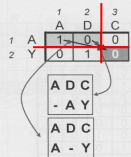
\includegraphics[width=0.3\textwidth]{figures/tre.png}
    \item Procediamo analogamente: ad esempio, verso (4,4)\\
    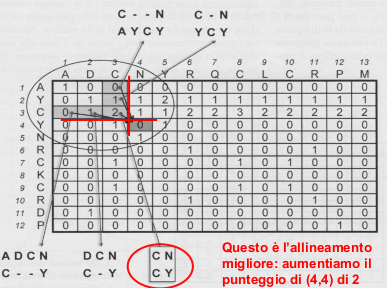
\includegraphics[width=0.6\textwidth]{figures/quattro.png}
    \item e oltre, ad es. verso (4,5): qui il nuovo punteggio sarà 3\\
    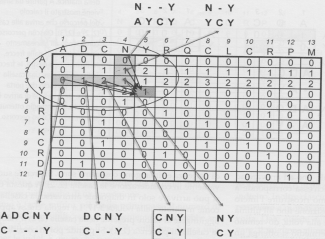
\includegraphics[width=0.6\textwidth]{figures/cinque.png}
    \item Alla fine arriveremo fino all'ultima casella in basso a dx:\\
    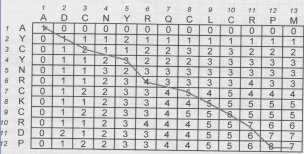
\includegraphics[width=0.6\textwidth]{figures/sei.png}
    \item Da essa possiamo spostarci a ritroso poiché abbiamo
    memorizzato i migliori punteggi dalle caselle precedenti.
    Abbiamo così determinato il miglior allineamento:\\
    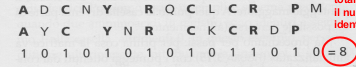
\includegraphics[width=0.8\textwidth]{figures/sette.png}
    \subitem \textit{Qui il punteggio totale coincide con il numero di residui
    identici.\\ ${8 \over 15} = 0.53 = 53\%$ identità di sequenza}
\end{enumerate}
\paragraph{In termini formali \dots} La casella (i,j) avrà lo score S(i,j)
ricalcolato a partire dalla matrice di inizializzazione in questo
modo:
\begin{center}
    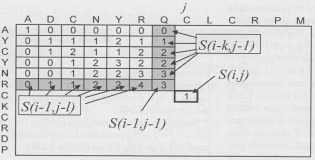
\includegraphics[width=0.6\textwidth]{figures/otto.png}
    $$ S(i,j) = {s(a,b) + max[S(i-1,j-1),S(i-k,j-1),S(i-1,j-l)]}$$
\end{center}
Dovremmo però trovare un modo più efficace di inizializzare la
matrice tenendo conto della similarità fra aa.
\subsection{Needleman-Wunsch: programmazione dinamica}
NW garantisce l'ottimalità dell'allineamento, anche se l'algoritmo non
calcola tutti i possibili allineamenti.
È un esempio di un algoritmo di programmazione dinamica:
un percorso ottimale (allineamento) è identificato dall'estensione
graduale di sottopercorsi localmente ottimali.
Dunque, una serie di decisioni è effettuata ad ogni passo
dell'allineamento per trovare la coppia di residui con il miglior
punteggio per quel passo.\\
L'algoritmo di Needleman-Wunsch è disponibile presso
EBI, che ospita molti tools per allineamenti locali e globali di
sequenze (Pairwise Sequence Alignment).

\begin{titlepage}
    \begin{center}
        \vspace*{1cm}
        \LARGE
        \textbf{Lezione 4: Allineamenti di Sequenze 2\\Matrici di Sostituzione}

    \end{center}
\end{titlepage}
\section{Waterman-Smith}
Un problema dell'algoritmo di Needleman-Wunsch: non si
tiene conto della penalizzazione delle indel.\\
L'algoritmo di WATERMAN-SMITH (1976) introduce
una funzione di penalizzazione delle indel, per migliorare
l'algoritmo NW, serve un sistema di pesatura delle indel, ad esempio:
$$ w(k) = g + e(k-1)$$
Il peso $w$ di una indel di lunghezza $k$ dipende dalla
penalizzazione per l'apertura di una singola indel ($g$) e
dalla penalizzazione per l'allungamento ($e$).
\subsection{L'algoritmo}
Nella pratica l'algoritmo procede in questo modo:
\begin{enumerate}
    \item nserisce una riga e una colonna 0-ime alla matrice
    di inizializzazione (calcolata ad esempio partire da
    BLOSUM o PAM che vedremo, ecco perché non ha
    solo 0 o 1). \\ Nella riga e colonna
    ombreggiate è
    sviluppata la funzione di
    penalizzazione: $w(k) = -12-4(k-1)$\\
    La riga e la colonna 0-sime contengono il
    punteggio che la
    sequenza avrebbe se
    allineata a una delezione
    lunga fino alla cella
    corrispondente.
    \item Tiene conto dei possibili modi per arrivare alla
    casella $(i,j)$. Il suo punteggio $S(i,j)$ dipende da essi:
    \begin{enumerate}
        \item Mi muovo in diagonale: no indel e
        punteggio dato da: punteggio
        della casella di partenza +
        punteggio della casella $(i,j)$
        secondo la matrice di
        inizializzazione (come in NW)
        \item Mi muovo in verticale o
        orizzontale: inserisco indel nella
        sequenza $i$ e $j$. Il punteggio sarà
        dato da: punteggio della casella
        di partenza - funzione di
        penalizzazione $w(k)$ ($k$ è la
        lunghezza della indel).
        \item Scelgo alla fine il percorso che dà
        il punteggio migliore
    \end{enumerate}
\end{enumerate}
\begin{center}
    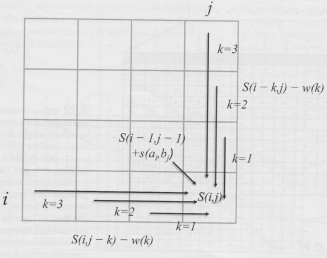
\includegraphics[width=0.5\textwidth]{figures/nw.png}
\end{center}
\section{Allineamento: globale vs locale}
\paragraph{Allineamento globale} (NW e SW visto finora) si estende da un
capo all'altro di ogni sequenza.
\paragraph{Allineamento locale} trova le regioni (sottosequenze) di due
sequenze che si allineano in modo ottimale.
\begin{center}
    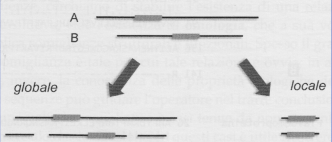
\includegraphics[width=0.5\textwidth]{figures/gl.png}\\
    \textit{Qui l'allineamento
    globale maschera la
    corrispondenza tra
    zone somiglianti}
\end{center}
SW si può modificare per renderlo capace di calcolare
allineamenti locali: basta introdurre fra i casi possibili $S(i,j)=0$ nel
caso in cui nell'allineamento globale fosse negativo
\paragraph{Esempio:} L'allineamento fra una
flavoemoproteina (con
un dominio di tipo
emoglobinico) e la
catena A
dell'emoglobina umana
\begin{itemize}
    \item \textbf{globale}: più difficile
    notare
    quantitativamente la
    similitudine
    \item \textbf{locale:} più apparente
\end{itemize}
\begin{center}
    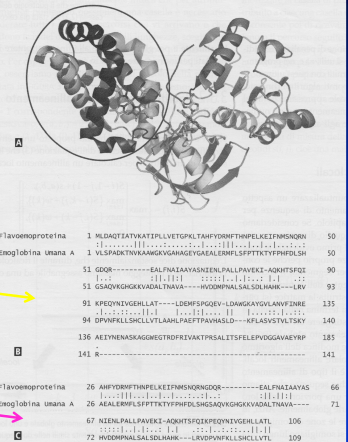
\includegraphics[width=0.5\textwidth]{figures/es1.png}\\
\end{center}
\paragraph{Esempio:} SW locale:dopo aver ricalcolato la matrice
cerco la cella con il valore massimo assoluto e parto da lì.\\
Gli stessi due peptidi di prima, allineati con Waterman-Smith
globale e locale danno luogo a matrici ed allineamenti
diversi. Partendo dalle caselle con score maggiore il
percorso a ritroso individua allineamenti differenti (non
sempre AL è sottoinsieme di AG)
\begin{center}
    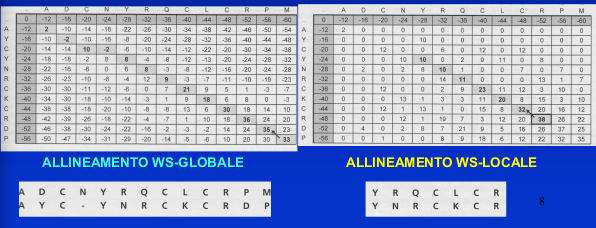
\includegraphics[width=0.5\textwidth]{figures/es2.png}\\
\end{center}
\subsubsection{In conclusione}
\begin{itemize}
    \item L'allineamento locale è quasi sempre utilizzato per il ricerche su
    database (tramite BLAST). E 'utile per trovare domini (o regioni
    limitate di omologia) all'interno di sequenze.
    \item Smith e Waterman (1981) hanno risolto il problema
    dell'allineamento locale ottimale di sequenze.
    \item Altri metodi (BLAST, FASTA) sono più veloci ma meno accurati.
    Li vedremo in seguito.
    \item In ogni caso, qualunque metodo di allineamento si scelga esso
    fornirà un punteggio S all'allineamento. Ricordiamo sempre che lo
    score S dipende dal metodo di allineamento e non è assoluto!
\end{itemize}
\subsection{Significatività statistica di un allineamento}
\paragraph{Domanda:}Ho allineato due sequenze A e B, ottenuto il punteggio S.
Come posso capire se sono omologhe? Che probabilità ho di
trovare il punteggio S “per caso”?\\
Il problema è più facilmente risolvibile per gli allineamenti
locali, e meno per quelli globali.
\subsubsection{Significatività allineamento globale: lo Z score}
La seq $A$ è mantenuta fissa; la $B$ è
“anagrammata” n volte ed ogni volta
globalmente allineata ad $A$, calcolando
lo score $S_i$ per l'allineamento $i$.
\begin{center}
    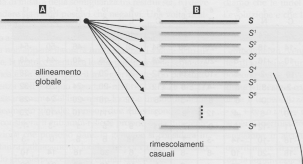
\includegraphics[width=0.5\textwidth]{figures/sig1.png}\\
\end{center}
$S_i$ si distribuisce su una curva di cui si
calcola la media $\mu$ e la deviazione
standard $\sigma$, Si definisce allora la
distanza $Z$ del punteggio $S$
dell'allineamento dalla media in termini
di dev. standard:
$$ Z = { S -\mu \over \sigma}$$
\begin{center}
    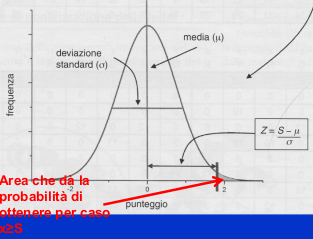
\includegraphics[width=0.5\textwidth]{figures/sig2.png}\\
\end{center}
\begin{center}
    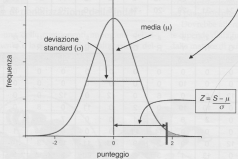
\includegraphics[width=0.5\textwidth]{figures/sig3.png}\\
\end{center}
\begin{itemize}
    \item Uno Z-score 0 = significa che la somiglianza osservata non è migliore
    rispetto alla media di permutazioni casuali della sequenza, e può anche
    essere casuale.
    \item Problema con Z-score: si assume una distribuzione normale, ma ciò
    può non esser corretto. Perciò Z deve essere considerato come una
    soglia di significatività.
\end{itemize}
\subsubsection{Significatività allineamento locale}
Teoria abbastanza complessa, sviluppata da Karlin e Altschul partendo da questa
osservazione:\\
Date due sequenze casuali, di lunghezza $m$ ed $n$, il numero atteso $E$ di
sottosequenze allineate localmente senza indel che ottengono un punteggio $S \geq x$ è:
$$E(S \geq x) = Kmne^{-\lambda x}$$
\begin{center}
    $m,n$ : lunghezze delle due sequenze.\\
    $K$: dipende dalla matrice di punteggio.\\
    $\lambda$: dipende dalla composizione amminoacidica.
\end{center}
Dalla definizione di $E$ si può calcolare la probabilità di osservare un
allineamento locale con punteggio $S \geq x$:
$$p(S \geq x) = \ - exp(Kmne^{- \lambda x})$$
Distribuzione del valore estremo o di Gumbel: è diversa dalla gaussiana
\begin{center}
    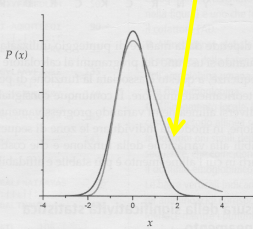
\includegraphics[width=0.5\textwidth]{figures/E.png}\\
\end{center}
In pratica:
\begin{itemize}
    \item allineamo localmente due seq
    \item otteniamo il punteggio $x$
    \item calcoliamo $p(S \geq x)$, la probabilità di
    ottenere un punteggio maggiore di $x$
    nell'ipotesi: le due seq NON sono
    omologhe
    \item se $p < $ soglia (es. 0.01 = 1\%) siamo
    confidenti che siano omologhe.
    \item SEMPRE: serve significatività
    BIOLOGICA oltre che statistica
\end{itemize}
\section{Matrici di punteggio}
Abbiamo già visto che per dare un punteggio a un allineamento
dobbiamo misurare la similitudine fra aa.
Usiamo perciò matrici di punteggio o di sostituzione: saranno
matrici $20x20$. Sono matrici simmetriche: $A \rightarrow B = B \rightarrow A$ (non
sappiamo evolutivamente chi si è trasformato dei due).
\paragraph{Come quantificare la somiglianza degli amminoacidi}
Difficile stabilire criteri oggettivi per le somiglianze fisico-chimiche
degli amino acidi. Non è possibile sapere a priori quali delle varie
caratteristiche fisico-chimiche sono più importanti per le proteine.\\
Emile Zuckerkandl e Linus Pauling (1965) considerarono
frequenze di sostituzione in 18 globine (mioglobine e
emoglobine da uomo a lampreda).
\begin{itemize}
    \item Nero: identità
    \item Grigio: sostituzione molto conservativa (occorrenza$>40\%$)
    \item Bianco: sostituzione abbastanza conservativa (occorrenza $> 21 \%$)
    \item Rosso: non è possibilte osservare sostituzioni
\end{itemize}
\begin{center}
    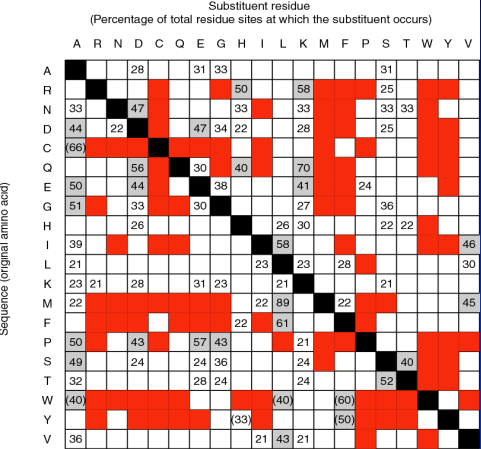
\includegraphics[width=0.5\textwidth]{figures/matx.png}\\
\end{center}
\paragraph{Cosa vogliamo ottenere?} una matrice (PAM250) di score.
Matrice di calcolo che assegna i
punteggi e tollera le discordanze.
Inoltre \dots tutta una serie di matrici di
punteggio, (fino a PAM10) che
è via via meno tollerante con i
disallineamenti.
\subsection{PAM: Point Accepted Mutation}
Mutazione puntuale accettata.
\begin{itemize}
    \item È l'evento in cui il DNA subisce una mutazione che produce il
    cambiamento di un aminoacido
    \item Tale mutazione diviene prevalente in una specie
\end{itemize}
Dayhoff ha osservato famiglie di sequenze identiche all'85\%
(omologhe e molto simili). Le ha allineate e ha creato alberi di
sequenze in cui ha dedotto le sequenze dei progenitori.
Piccoli passi evolutivi, per osservare l'evoluzione e dedurne le
caratteristiche.\\
Le matrici PAM sono basate su allineamenti globali di
proteine strettamente correlate. Il PAM1 è la matrice calcolata dal confronto di sequenze con
non più di 1\% di divergenza. Ad un intervallo evolutivo di
PAM1, un cambiamento si è verificato su una lunghezza di
100 aminoacidi.\\
Altre matrici PAM sono estrapolate da PAM1 ( PAM1 non ha
utilità pratica ). Per PAM250, 250 sostituzioni si sono verificate
tra due proteine su una lunghezza di 100 aminoacidi, nel
passo evolutivo che essa rappresenta.\\
\textit{Nota bene:}Tutti i dati PAM provengono da proteine
strettamente correlate ($>$ 85\% di identità degli aminoacidi).
\newpage
\paragraph{Dayhoff: 34 superfamiglie di proteine}
\begin{center}
    \begin{tabular}{c|c}
        \toprule
        \textbf{Proteina} & \textbf{PAMs per 100 milioni di anni}\\
        \midrule
        Ig kappa chain & 37 \\
        Kappa casein & 33 \\
        luteinizing hormone b & 30 \\
        lactalbumin & 27 \\
        complement component 3 & 27 \\
        epidermal growth factor & 26\\
        proopiomelanocortin & 21\\
        pancreatic ribonuclease & 21 \\
        haptoglobin alpha & 20 \\
        serum albumin & 19 \\
        phospholipase A2, group IB & 19 \\
        prolactin & 17 \\
        carbonic anhydrase C & 16 \\
        Hemoglobin $\alpha$ & 12\\
        Hemoglobin $\beta$ & 12 \\
        apolipoprotein A-II & 10\\
        lysozyme & 9.8 \\
        gastrin & 9.8 \\
        myoglobin & 8.9 \\
        nerve growth factor & 8.5 \\
        myelin basic protein & 7.4 \\
        thyroid stimulating hormone b & 7.4 \\
        parathyroid hormone & 7.3 \\
        parvalbumin & 7.0 \\
        trypsin & 5.9 \\
        insulin & 4.4 \\
        calcitonin & 4.3 \\
        arginine vasopressin & 3.6 \\
        adenylate kinase & 3.2 \\
        triosephosphate isomerase 1 & 2.8 \\
        vasoactive intestinal peptide & 2.6 \\
        glyceraldehyde phosph. dehydrogease & 2.2 \\
        cytochrome c & 2.2 \\
        collagen & 1.7 \\
        troponin C, skeletal muscle & 1.5 \\
        alpha crystallin B chain & 1.5 \\
        glucagon & 1.2 \\
        glutamate dehydrogenase & 0.9 \\
        histone H2B, member Q & 0.9 \\
        ubiquitin & 0
    \end{tabular}
\end{center}
\begin{center}
    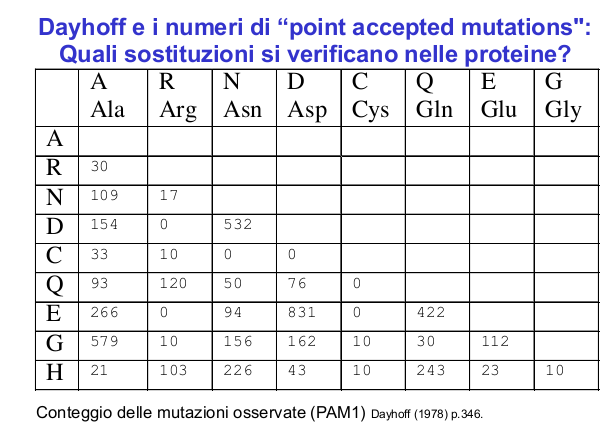
\includegraphics[width=0.5\textwidth]{figures/dayhoff2.png}\\
\end{center}
\subsection{La mutabilità relativa degli amminoacidi}
\paragraph{Quanto spesso mutano nelle proteine?}
Definiamo la Frequenza relativa di mutazione.
\begin{center}
    \begin{tabular}{c | c !{\vline width 2pt} c | c }
        \toprule
        \textbf{AA} & \textbf{Freq} & \textbf{AA} & \textbf{Freq}\\
        \midrule
        Asn & 134 & His & 66 \\
        Ser & 120 & Arg & 65 \\
        Asp & 106 & Lys & 56 \\
        Glu & 102 & Pro & 56 \\
        Ala & 100 & Gly & 49 \\
        Thr & 97 & Phe & 41 \\
        Ile & 96 & Phe & 41 \\
        Gln & 93 & Cys & 20 \\
        Val & 74 & Trp & 18 
    \end{tabular}
\end{center}
\paragraph{Frequenze normalizzate}
\begin{center}
    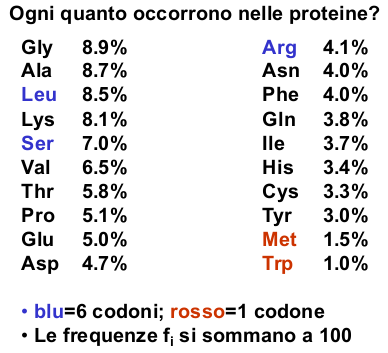
\includegraphics[width=0.5\textwidth]{figures/norm.png}\\
\end{center}
\paragraph{Esempio}
Prendiamo un allineamento multiplo di sequenze,
ad esempio della deidrogenasi gliceraldeide 3-fosfato.\\
\textbf{OSSERVAZIONE:}
le colonne di residui possono avere conservazione alta o bassa.
\begin{center}
    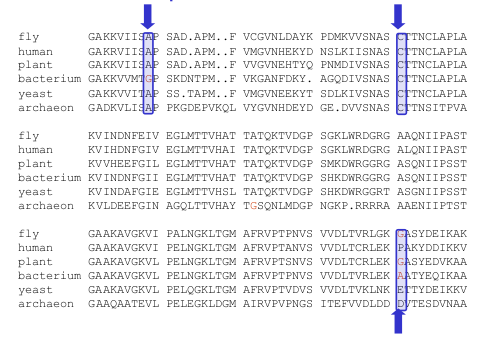
\includegraphics[width=0.5\textwidth]{figures/es3.png}\\
\end{center}
\subsubsection{Matrice PAM1 (probabilità) di Dayhoff}
\begin{center}
    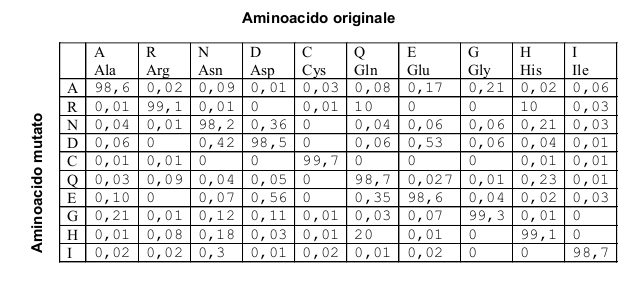
\includegraphics[width=0.5\textwidth]{figures/pam1.png}\\
\end{center}
Ogni elemento della matrice mostra la probabilità che un
amminoacido (in alto) venga sostituito da un altro aminoacido
(a lato).
\section{Matrici di sostituzione}
Una matrice di sostituzione contiene valori proporzionali
alla probabilità che l'amminoacido i muti nell' amminoacido $j$
per tutte le coppie possibili di aminoacidi. Le matrici di sostituzione sono costruite assemblando
un campione ampio e diversificato di allineamenti a coppie
(o allineamenti multipli di sequenza) di aminoacidi.\\
Le matrici di sostituzione dovrebbero riflettere la probabilità
reale di mutazione in un periodo di evoluzione.
I due principali tipi di matrici di sostituzione: PAM e BLOSUM.
\subsection{Moltiplicare le matrici}
Con (PAM1)$^\wedge$n si può simulare il passaggio di n passi di
evoluzione.
\begin{center}
    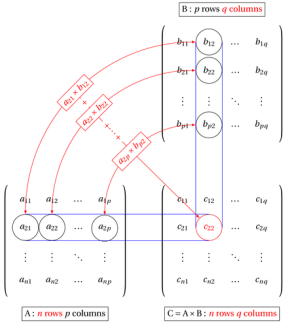
\includegraphics[width=0.5\textwidth]{figures/pamn.png}\\
\end{center}
\paragraph{Matrice di sostituzione PAM0 (probabilità)} Ovvero: nulla cambia.
\begin{center}
    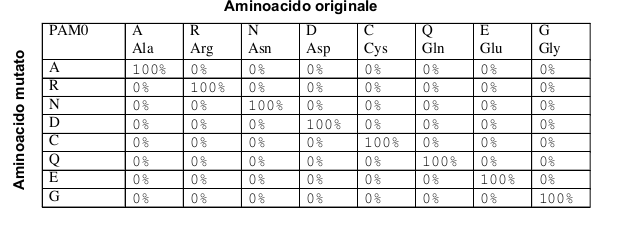
\includegraphics[width=0.5\textwidth]{figures/pam0.png}\\
\end{center}
Si sono verificati 0 passi di evoluzione: non è cambiato nulla!
\paragraph{Matrice di sostituzione PAM2000 (probabilità)} PAM1$^\wedge$2000, ovvero: il caso.
\begin{center}
    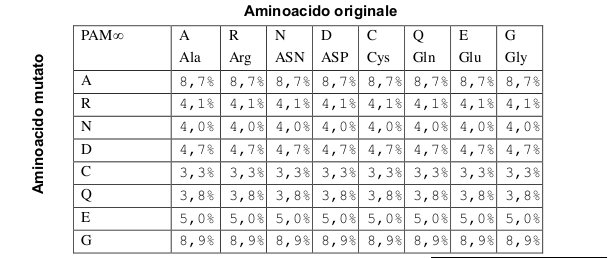
\includegraphics[width=0.5\textwidth]{figures/pam2000.png}\\
\end{center}
Moltiplicando PAM1 per 2000 (passi di
evoluzione)si arriva ad una situazione in cui la
probabilità converge alla frequenza osservata
\paragraph{Matrice di sostituzione PAM250 (probabilità) di mutazione} 
\begin{center}
    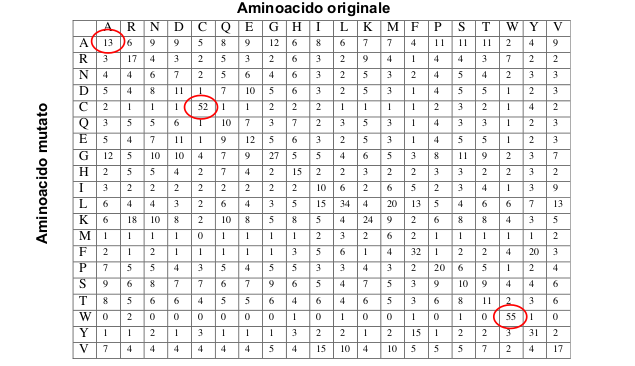
\includegraphics[width=0.5\textwidth]{figures/pam250.png}\\
\end{center}
PAM 250 è un caso interessante: ottenuta da PAM1$^\wedge$250 prevede che circa il 20\%
della sequenza sia conservato. A $ \rightarrow$ A ha probabilità del 13\%. Da notare W e C che
anche dopo 250 mutazioni hanno il 50\% di probabilità di non mutare.

\begin{titlepage}
    \begin{center}
        \vspace*{1cm}
        \LARGE
        \textbf{Lezione 6: Allineamenti Multipli di Sequenze}

    \end{center}
\end{titlepage}
\section{Allineamento multiplo di sequenze}
\subsection{Visione Generale}
\subsubsection{Una definizione}
Un allineamento multiplo è una collezione di tre o più sequenze proteiche (o nucleotidiche) parzialmente o completamente allineate
\begin{itemize}
    \item I residui e le zone omologhe sono allineate in colonne per tutta la lunghezza delle sequenze
    \item Il senso dell'omologia dei residui è evoluzionistico
    \item Il senso dell'omologia dei residui è strutturale
\end{itemize}
Si tratta di un argomento di ricerca attivo dagli anni '90.
\subsubsection{Alcuni fatti}
Non c'è necessariamente un allineamento "corretto" per una famiglia di proteine.\\
\textbf{Perchè?}
    \begin{itemize}
        \item Le sequenze di proteine evolvono
        \item Le corrispondenti strutture tridimensionali evolvono, anche se più lentamente
        \item Può essere particolarmente difficile identificare i residui che si sovrappongono nello spazio (strutturalmente) in un allineamento multiplo di sequenze.
    \end{itemize}
\hl{Due proteine che condividono il 30\% di identità di sequenza avranno circa il 50\% dei residui sovrapponibili nelle due strutture}
\subsubsection{Caratteristiche utili per realizzzarlo}
Alcuni residui allineati, come cisteine che formano ponti disolfuro, o i triptofani, possono essere altamente conservati
    \begin{itemize}
        \item Ci possono essere motivi conservati come un dominio transmembrana
        \item Alcune caratteristiche come le strutture secondarie, siti attivi e di legame per ligandi o complessi sono spesso conservate
        \item Ci possono essere regioni con inserimenti o delezioni propagati in parte della famiglia.
        \item I principi che vedremo sono focalizzati sulle proteine ma sono validi in generale anche per sequenze nucleotidiche.
    \end{itemize}
\subsubsection{Utilizzi e Vantaggi}
    \begin{itemize}
        \item Il MSA è più sensibile di quello a coppie nel rilevamento di omologie, per questo è uno strumento essenziale nella costruzione di modelli strutturali per omologia
        \item L'output di BLAST può assumere la forma di un MSA, e possono essere individuati residui conservati o motivi
        \item In un MSA si possono analizzare i dati di una popolazione
        \item Una singola query può essere cercata contro un database di MSA (ad esempio Pfam)
        \item Le regioni regolatorie dei geni sono spesso identificabili da MSA
    \end{itemize}
\subsection{Metodi}
I metodi esatti non vengono trattati in questa sede: non ci sono soluzioni efficienti e già con 5 sequenze il tempo di computazione è eccessivo (esponenziale)
\subsubsection{Metodi Euristici}
\hl{\textbf{Metodi progressivi}}: usano un albero guida (analogo ad un albero filogenetico) per determinare come combinare uno per uno allineamenti a coppie
(progressivamente) per creare un allineamento multiplo.\\
\small{Esempi: CLUSTAL OMEGA (W), MUSCLE (usato da HomoloGene)}
\paragraph{Il MSA progressivo di Feng-Doolittle (1987) alla base di Clustal (W) avviene in 3 fasi}
\begin{enumerate}
    \item Realizzare una serie di allineamenti a coppie globali (Needleman e Wunsch, algoritmo di programmazione dinamica) di cui si calcola la distanza (matrice delle distanze)
    \item Creare un albero guida a partire dalla matrice delle distanze
    \item Allineare progressivamente le sequenze
\end{enumerate}
\textbf{MSA progressivo, fase 1 di 3:}\\
\normalsize{generare allineamenti a coppie globali}\\
\small{Esempio: allineare 5 globine (1, 2, 3, 4, 5).}\\
\paragraph{\hl{Primo step:} a due a due e valutare gli score di ogni possibile allineamento a coppie\\}
\textbf{Numero di allineamenti a coppie necessari per coprire tutte le possibili combinazioni}
\begin{itemize}
    \item Per n sequenze, (n-1) (n) / 2
    \item Per 5 sequenze, (4) (5) / 2 = 10
    \item Per 200 sequenze, (199) (200) / 2 = 19.900
\end{itemize}…Quindi per molte sequenze ClustalW è molto lento ed è preferibile usare metodi più veloci (MUSCLE è molto veloce).
\paragraph{\hl{Secondo step:} albero guida\\}
\textbf{Convertire i punteggi di similitudine in punteggi di distanza:} è matematicamente più semplice, oltre che più intuitivo, lavorare con le distanze. Una semplice definizione di distanza è data dalla percentuale di
residui diversi (100- SI in \%) che viene inserita nella matrice delle distanze.
\begin{itemize}
    \item Dalla matrice delle distanze si calcola l'albero guida con il metodo di clustering neighbor joining che vedrete nel modulo 2.
    \item Vediamo un semplice esempio di clustering e costruzione di albero guida
\end{itemize}
\paragraph{Il clustering alla base di CLUSTAL(W)} È una matrice di distanze, minore è il numero, maggiore è la similitudine.
\textit{Nota: tutte le distanze tra la I e la IV riga sono minori di quelle riportate nella V}
%inserire foto 
\begin{itemize}
    \item Tutte le sequenze vengono poi allineate progressivamente, seguendo le indicazioni dell'albero
    guida: prima si allineano le più simili (vicine) e poi progressivamente le più distanti.
    \item A ogni passaggio si utilizza un algoritmo dinamico di allineamento molto efficiente che accoppia sequenze o gruppi di sequenze
    \item Il MA è composto a partire a tanti allineamenti a coppie, anche fra gruppi di sequenze.
    \item{} \textit{Nota: Le indel presenti negli allineamenti già effettuati restano fisse.}
    \item Come allineare pogressivamente due gruppi di sequenze? Si usa sempre una matrice. È simile all'allineamento dinamico di due sequenze visto.
    \item Lo score S in ogni
    casella è la media degli score ottenuti confrontando tutte le possibili coppie di a.a. nella riga e colonna
    corrispondenti (secondo ad es. BLOSUM62)
    \item 
\end{itemize}


\begin{titlepage}
    \begin{center}
        \vspace*{1cm}
        \LARGE
        \textbf{Domande stile esame}

    \end{center}
\end{titlepage}

\section{Domande sull'introduzione}
\Large
\begin{enumerate}
    \item Differenza tra omologia e similitudine. È possibile che due proteine abbiano unìidentità di sequenza del 57\% e una similitudine del 21\%? Perchè?
\end{enumerate}

\section{Domande sulle banche dati}
\begin{enumerate}
    \item ) Cos'è Uniprot? Oltre ad una descrizione generale si descrivano i suoi livelli e si elenchino almeno 5 sezioni che si possono trovare nelle pagine delle singole proteine (entry). Si descrivano inoltre brevemente i database PDB e ExPASy. Cosa hanno in comune queste tre risorse?
    \item Si citino e discutano brevemente 4 banche dati presenti in NCBI. Se possibile escludere NCBI protein.
    \item Si descrivano le banche dati NCBI Gene, Unigene e Genbank. Inoltre, in che relazione sono tra di esse?
    \item  Descrivere Uniprot, Pfam, Prosite, CATH e PDB, con particolare attenzione alla più importante tra di esse (qual è?)
    \item Cos'è Pubmed? Descrivere la banca dati, i suoi contenuti, e gli strumenti messi a disposizione degli utenti (illustrati a lezione), sia per la ricerca che per la gestione dei risultati.
    \item Descrivere brevemente le caratteristiche del Protein Data Bank ed il contenuto di un file pdb.
    \item Si descrivano il formato FASTA, il formato ASN.1 e il formato XML nell'ambito della bioinformatica.
    \item 
\end{enumerate}


\end{document}